\documentclass{article}
\usepackage{amsmath,amssymb}
\usepackage[margin=1in]{geometry}
\usepackage{tikz}
\usetikzlibrary{positioning}

\newcommand{\CC}{\mathcal{C}}
\newcommand{\NN}{\mathcal{N}}
\newcommand{\union}{\cup}


\begin{document}

\title{Regularising a CCD to full support}
\author{Yang, Bouckaert, Drummond}
\date{}
\maketitle

A conditional clade distribution (CCD) assigns probability zero to any tree
containing a clade or split its sample never produced. For held-out evaluation
and for use as a tree prior this is too brittle: an independent posterior sample
routinely visits trees just outside the support. We want a regulariser that gives
\emph{every} tree nonzero probability while keeping the observed structure sharp,
and that places the right amount of mass on the unseen region. Here we develop a full-support, single-parameter regulariser that computes the probability of novelty at lazily without
enlarging the clade set. Appendix~A records an earlier route, NNI clade expansion,
which enlarges the clade set by a fixed local move-set; the main model
subsumes its coverage with a simpler construction.

\section*{CCD regularisation: full support from a single parameter}

\paragraph{Motivation.}
One way to give unsampled clades nonzero probability is to \emph{enlarge the clade
set} with the clades reachable by a fixed local move (NNI clade expansion;
Appendix~A). Such an approach has three problems: it \emph{mutates the
graph} (a clade-enumeration pass plus a second split expansion), it adds extra parameters
$(\beta,\text{mode})$ on top of $\alpha$, and it covers only the novelty its
move-set can reach so that trees more than one NNI from the support still receive
probability zero. The construction we prefer instead computes a probability of unsampled clades on demand without touching the sampled clade set, gives
\emph{every} tree nonzero probability, and is governed by a single parameter
$\mu$, the per-clade probability of escaping the sampled splits.

\paragraph{Red/blue decomposition.}
Keep the split-expanded, additive-$\alpha$ backbone of \eqref{eq:smoothing}, but
add \emph{no} clades. To score a tree $T$, colour each internal node \emph{red} if
its split is present in the (expanded) CCD and \emph{blue} otherwise; a blue node
necessarily involves an unobserved clade. Blue nodes form maximal connected
\emph{regions}. The top of a region is always an observed clade $C$ (its parent is
red, or it is the root), and its boundary $\partial B$ is the set of $m$ observed
subclades hanging immediately below it (the first red or leaf nodes). Such a
region resolves $C$ into its $m$ boundary parts through exactly $m-2$ novel
intermediate clades.

\paragraph{Probability.}
Red nodes keep their smoothed conditional clade probability $\theta$, discounted
by a reserved escape mass $\mu$; each blue region is charged one factor of
$\epsilon$ per novel clade, spread uniformly over the ways its boundary can be
realised:
\begin{equation}
  P(T)=\prod_{v\in\mathrm{red}(T)}\!(1-\mu)\,\theta\!\left(S_v\mid C(v)\right)
       \;\prod_{B\in\mathrm{blue}(T)}\!\frac{\epsilon(C_B)^{\,m_B-2}}{\pi(C_B,\partial B)},
  \label{eq:blueregion}
\end{equation}
where $\pi(C,\partial B)$ (the \emph{pathcount}) is the number of all-novel
resolutions of $C$ into the boundary $\partial B$, computed by a subset
dynamic program over the at most $m$ parts. The division by $\pi$ makes the
reserved mass uniform over the unseen trees of a given boundary.

\paragraph{Per-clade reserve.}
The escape factor $\epsilon(C)$ is fixed per clade by requiring the blue mass to
equal a target escape probability $\mu$:
\begin{equation}
  R(C)=\sum_{j\ge 1} N_j(C)\,\epsilon(C)^{j}=\mu,
  \qquad
  N_j(C)=\#\Bigl\{\text{partitions of $C$ into $j{+}2$ observed subclades}\Bigr\},
  \label{eq:reserve}
\end{equation}
restricted to partitions admitting an all-novel resolution (the pathcount
cancellation in \eqref{eq:blueregion} collapses the resolutions, leaving one term
per partition). Thus $\mu$ is the per-clade probability of escaping the sampled
splits, and is the model's only free parameter; $\mu=0$ recovers the unsmoothed
backbone.

\paragraph{Full support by decoupling coverage from normalisation.}
Evaluating \eqref{eq:reserve} exactly is \#P-hard: $N_j(C)$ is a set-partition
count over the non-laminar clade family, growing as $O(m^{j+1})$ in the number $m$
of observed subclades of $C$. The key observation is that \emph{coverage does not
need it}. A tree receives nonzero probability as soon as (i) scoring is not
truncated, and (ii) $\epsilon(C)>0$ at each region top. Any region actually
present in $T$ is itself a valid novel partition, so $N_m(C)\ge 1$ and a positive
$\epsilon$ exists. The exact $N_j$ only fix the \emph{value} of $\epsilon$. We
therefore solve \eqref{eq:reserve} from the cheap low orders alone (reserve depth
$k$; $N_1$ is $O(m^2)$, $N_2$ is $O(m^3)$) and score regions of \emph{every}
depth with that $\epsilon$. The result is full support based on a low-order approximation of $\epsilon(C)$ per sampled clade: every tree, at any novelty depth, is covered.

\paragraph{Normalisation and a non-inflating guarantee.}
Scoring all orders based on a depth-$k$ estimate of $epsilon(C)$ will assign slightly too much probability mass to trees that escape the CCD at clade C by omitting the tail, so the model is slightly \emph{super}-normalised. This 
\emph{inflates} the held-out log-probabilities and overestimates the fit of the model in any held-out
comparison. The defect is
\begin{equation}
  \mathrm{tail}(C)=\sum_{j>k}N_j\,\epsilon^j
  \;\le\; N_2\,\epsilon^2\,\frac{\rho}{1-\rho},
  \qquad \rho=\frac{N_2}{N_1}\,\epsilon,
  \label{eq:tail}
\end{equation}
a geometric upper bound read straight off the two computed orders (rigorous when
the $N_j$ are log-concave), scaling as $\mu^{k+1}/m^{k}$. Discounting red splits by
$1-\mu-\mathrm{tail}(C)$ instead of $1-\mu$ guarantees the total probability can be at most
$1$: the model is then \emph{sub}-normalised and can never over-state the model fit. A
Knuth backtrack-tree estimate of the tail gives the near-exact value instead of
the bound. On RSV2 the inflation scales as $\mu^3$ and is negligible for realistic posterior samples, becoming material only for large $\mu$:
\begin{center}
\renewcommand{\arraystretch}{1.1}
\begin{tabular}{lrr}
\hline
$\mu$ & true inflation (sampled) & upper bound \\
\hline
$0.01$ & $0.0001$ & $0.0001$ \\
$0.05$ & $0.0007$ & $0.0101$ \\
$0.10$ & $0.014$ & $0.077$ \\
$0.20$ & $0.116$ & $0.662$ \\
\hline
\end{tabular}
\end{center}
(mean nat/tree on held-out RSV2). A safety check warns whenever $\mu>0.05$, beyond
which the bound exceeds $\sim 0.01$ nat/tree.

\paragraph{RSV2.}
Under $5$-fold leave-one-tree-out on the strict-clock posterior ($n=129$, $2{,}251$
trees, backbone $\alpha=0.4$, $\mu=0.01$), the blue-region model covers every
held-out tree at mean held-out log-probability competitive with the tuned
graph-wide NNI of Appendix~A:
\begin{center}
\renewcommand{\arraystretch}{1.1}
\begin{tabular}{lrr}
\hline
model & coverage & mean $\log P$ (common set) \\
\hline
regCCD (no clade expansion) & $89.6\%$ & $-53.50$ \\
NNI clade expansion (co-occurring) & $99.3\%$ & --- \\
KRegCCD, ($\mu=0.01$) & $\mathbf{100.0\%}$ & $-54.20$ \\
\hline
\end{tabular}
\end{center}
Full support guarantees the $100\%$ structurally rather than by enlarging a clade
set; the residual that NNI co-occurring misses (novelty an SPR-move away) is
covered here automatically. The common-set log-probabilities are over the trees
all models cover (the $\sim 90\%$ within plain regCCD's support), on which regCCD
is marginally sharper precisely because it reserves no escape mass there; the
blue-region model trades that fraction of a nat to cover the remaining $\sim 10\%$
of held-out trees that contain a novel clade, which regCCD assigns probability
zero.

\paragraph{Calibration: the right amount of novelty.}
Because $\mu$ is the only parameter and directly governs the escape mass, the model's
total probability on trees that contain a novel clade has a closed form,
\begin{equation}
  P(\text{novel})=1-M(\rho),\qquad
  M(c)=\bigl(1-\mu\bigr)^{[c\ \text{reserves}]}
        \!\!\!\sum_{(L,R)\in S^{\mathrm{obs}}(c)}\!\!\! \theta(L,R)\,M(L)\,M(R),
  \label{eq:pnovel}
\end{equation}
the mass that stays entirely within the observed clade set ($M=1$ on leaves; the
$(1-\mu)$ factor applies at clades large enough to host an escape). Training on one
half of the strict-clock posterior and scoring the independent held-out half, we
compare \eqref{eq:pnovel} against the \emph{empirical} fraction of held-out trees
that actually contain a novel clade ($0.214$ here because the modest training sample
makes this a high-novelty regime). Mean log-probability is over \emph{all}
held-out trees (the model covers them all), so it sits below the common-set value
of the table above.
\begin{center}
\renewcommand{\arraystretch}{1.1}
\begin{tabular}{lrrrr}
\hline
$\mu$ & model $P(\text{novel})$ & empirical & ratio & mean $\log P$/tree \\
\hline
$0.002$  & $0.132$ & $0.214$ & $0.62\times$ & $-56.953$ \\
$0.003$  & $0.192$ & $0.214$ & $0.90\times$ & $-56.869$ \\
$0.0035$ & $0.220$ & $0.214$ & $1.03\times$ & $-56.846$ \\
$\mathbf{0.004}$  & $\mathbf{0.247}$ & $0.214$ & $\mathbf{1.15\times}$ & $-56.830$ \\
$0.005$  & $0.299$ & $0.214$ & $1.40\times$ & $\mathbf{-56.816}$ \\
$0.006$  & $0.347$ & $0.214$ & $1.62\times$ & $-56.818$ \\
$0.010$  & $0.509$ & $0.214$ & $2.38\times$ & $-56.907$ \\
\hline
\end{tabular}
\end{center}
The mean held-out log-probability has an interior optimum (too small a $\mu$ starves
the genuinely novel trees, too large dilutes the observed ones), and is \emph{flat}
across $\mu\in[0.004,0.006]$, all within $\sim 0.005$ nat of the peak at $\mu=0.005$.
The operating point can therefore be chosen for calibration at essentially no cost in
sharpness: at $\mu\approx 0.004$ the model places mass on novel-clade trees within
$\sim\!1.15\times$ of the empirical rate (exact calibration, $1.03\times$, at
$\mu\approx 0.0035$), giving up only $\sim 0.01$ nat against the sharpness peak. A
single parameter, pinned inside a flat held-out-likelihood plateau, thus delivers
both full coverage and the right amount of mass on the unseen region. This is the
blue-region counterpart of the factor-$1.2$ calibration that
Appendix~A obtains from the two-parameter $(\alpha,\beta)$ smoothing, here from one
parameter and the closed-form recursion \eqref{eq:pnovel}.

\paragraph{Why this is preferred.}
The blue-region construction matches the NNI expansion's coverage and sharpness
while being strictly simpler and more general:
\begin{itemize}
  \item \textbf{One parameter.} A single escape probability $\mu$ replaces
    $(\alpha_{\text{NNI}},\beta,\text{mode})$; the backbone $\alpha$ is the only
    other parameter and is shared with plain regCCD.
  \item \textbf{No graph mutation.} The clade set is untouched so there is no clade
    enumeration, no second split expansion.
  \item \textbf{Full support.} Every tree has nonzero probability, not only those
    within a fixed move-set, so coverage is not capped at NNI (or any) rearrangement
    depth.
  \item \textbf{Coverage is free.} It is decoupled from the \#P-hard exact
    normalisation: $100\%$ coverage needs only the $O(m^3)$ low-order estimate to high accuracy for low $\mu$.
  \item \textbf{Controlled normalisation.} The tail correction makes the
    normalisation explicit and either provably non-inflating or near-exact.
\end{itemize}


\clearpage

\appendix

\section*{Appendix A: clade-level NNI expansion}

\paragraph{Motivation.}
The CCD0 construction \emph{expands the split set}: for every clade partition
$P\to\{L,R\}$ that could exist because its parent $P$ and both children $L,R$ are
already clades in $\CC$ (the set of clades with nonzero marginal support), it
adds that partition even if no sampled tree realised it. Here we describe the
analogous operation one level up (expanding the \emph{clade set} $\CC$ itself)
by reading nearest-neighbour-interchange (NNI) rearrangements directly off
the stored splits, without ever building a tree.

\paragraph{NNI at the clade level.}
An internal edge of a tree is a stored split $P\to\{L,R\}$: the parent clade $P$
branches into disjoint children $L,R$ with $L\union R=P$. An NNI at that edge
needs the grandchildren. Descend into one child, say $L$, with its split
$L\to\{A,B\}$, and let the sibling be $R$. The three subtrees meeting at the edge
are $A$, $B$, $R$. The two NNI moves recombine them so that the child of $P$ is no
longer $L=A\union B$ but
\begin{equation}
  A\union R \qquad\text{or}\qquad B\union R .
  \label{eq:recomb}
\end{equation}
Because $A\subseteq L$ and $L\cap R=\varnothing$, each union in
\eqref{eq:recomb} is a disjoint union of size $\ge 2$ and a \emph{proper}
subclade of $P$ (it omits the nonempty $B$ resp.\ $A$). Each novel clade carries
an NNI-implied \emph{seed split}
\[
  (A\union R)\to\{A,R\},
\]
whose two constituents $A,R$ are themselves clades already in $\CC$. The roles of
$L$ and $R$ are symmetric, so a split $R\to\{C,D\}$ likewise yields $C\union L$
and $D\union L$. Every quantity ($A,B,R$ and the parent $P$) is read
straight from the CCD's split table.

\paragraph{Algorithm.}
For each clade $P$ with $|P|\ge 3$, each split $\{L,R\}\in\Pi(P)$, each choice of
descend-child $X\in\{L,R\}$ with sibling $Y$, and each grandchild split
$\{A,B\}\in\Pi(X)$, emit the candidates $A\union Y$ and $B\union Y$; keep those
not already in $\CC$. This is a pass over pairs of adjacent splits, costing
\[
  O\!\Big(\textstyle\sum_{P} |\Pi(P)|\cdot \max_{X}|\Pi(X)|\Big)
  \;=\; O\big(|\text{splits}|\times \bar{d}\big),
\]
with $\bar d$ the average number of splits per clade, proportional to the size
of the CCD, not to the number of trees it represents.

\paragraph{Two pairing modes.}
The CCD graph mixes splits from many posterior trees, so the algorithm above can
combine a split $P\to\{L,R\}$ with a grandchild split $L\to\{A,B\}$ that never
occurred together in any one tree. We therefore distinguish:
\begin{itemize}
  \item \textbf{Graph-wide} ($\NN_{\mathrm{gw}}$): pair \emph{any} stored split on
    $P$ with \emph{any} stored split on its child $X$. Cheapest and broadest; the
    pass described above.
  \item \textbf{Co-occurring} ($\NN_{\mathrm{co}}$): only recombine grandchild
    splits that actually appeared together under $P$ in some single base tree,
    the true NNI neighbourhood of the posterior sample. This is obtained by
    walking the stored base trees and reading $A,B,R$ off each internal edge.
\end{itemize}
By construction $\NN_{\mathrm{co}}\subseteq\NN_{\mathrm{gw}}$: the co-occurring
set is the graph-wide set restricted to split pairs realised within a single
tree. The graph-wide extras are exactly the clades that \emph{no single sampled
tree is one NNI move away from}; whether that is desirable broader coverage or an
overreach beyond the sample's NNI neighbourhood is a modelling choice one should
state explicitly.

\paragraph{Conservativeness.}
NNI is the most local rearrangement, so the expansion recovers only clades
``near'' the support and misses anything requiring an SPR-scale move. For the
single tree $(((A,B),C),D)$ the expansion yields exactly $\{ABD, CD, AC, BC\}$;
it does \emph{not} produce $AD$, $BD$, $ACD$ or $BCD$, which need a non-local
move. If the concern is held-out trees that differ from the sample by a single
local rearrangement, this coverage is exactly right; for broader topological
novelty one would extend to SPR neighbourhoods, also expressible at the clade
level (a regrafted subtree clade unioned with whatever lies below the target
edge), at the cost of many more candidates.

\subsection*{A.1\quad Parameterisation in CCD1 / regCCD}

The clade expansion is most natural in the \emph{split}-parameterised models.
A regularised CCD (regCCD) takes the CCD1 graph, adds the unobserved splits whose
parent and children are already clades (the CCD0 split expansion), and prices
every split of a clade $C$ by additive smoothing,
\begin{equation}
  \theta_\alpha(S)=\frac{f(S)+\alpha}{f(C)+\alpha\,|S(C)|},
  \label{eq:smoothing}
\end{equation}
a $\mathrm{Dirichlet}(\alpha,\dots,\alpha)$ prior over the splits $S(C)$. This
gives nonzero probability to trees with \emph{unsampled splits of sampled
clades}, but a tree containing an \emph{unsampled clade} still has probability
zero: the residual limitation of both CCD0 and CCD1.

NNI clade expansion closes this gap, and, crucially, needs \emph{no new
parameter}. Under the CCD1 form $P(T)=\prod_v \mathrm{CCP}\!\left(\text{split}\mid
\text{clade}\right)$ a clade carries no marginal parameter; its probability is
induced by the product along the path to it. So adding a novel clade $K=A\cup R$
only requires its \emph{splits} to be in the graph:
\begin{itemize}
  \item the recombined parent split $P\to\{K,B\}$ enlarges $S(P)$ and is priced
    by \eqref{eq:smoothing} with $f=0$, i.e.\ mass $\alpha/(f(P)+\alpha|S(P)|)$;
  \item the seed split $K\to\{A,R\}$ (and any further splits of $K$ into existing
    clades found by the split expansion) is priced the same way; a clade left
    with a single split is deterministic ($\mathrm{CCP}=1$).
\end{itemize}
A held-out tree that is one NNI move from the support is then scored
$P(T)=\bigl[\prod\text{observed CCPs}\bigr]\cdot\theta_\alpha(P\to\{K,B\})\cdot
\theta(K\to\{A,R\})>0$. The novel clades enter the \emph{same} additive-$\alpha$
Dirichlet--multinomial as the observed and split-expanded splits (single
pseudocount), so the only model change is a larger clade set.

\paragraph{Coverage vs.\ sharpness, and a two-level prior.}
The benefit is out-of-sample coverage of trees with unsampled clades; the cost is
that enlarging $|S(P)|$ dilutes the smoothed mass of observed splits. The latter
is controlled by giving NNI-derived splits (those touching a novel clade) a
\emph{separate} pseudocount $\beta$, while observed and split-expanded splits keep
$\alpha$:
\begin{equation}
  \theta(S)=\frac{f(S)+\alpha\,[S\text{ regular}]+\beta\,[S\text{ NNI}]}
                 {f(C)+\alpha\,|R(C)|+\beta\,|N(C)|},
  \label{eq:twolevel}
\end{equation}
an asymmetric Dirichlet placing a weaker prior on the speculative
recombinations. Crucially $\beta$ does not affect \emph{coverage} (any
$\beta>0$ keeps the NNI split positive); it only rebalances mass at observed
parents.

\paragraph{Choosing the pseudocounts.}
Since $\beta$ does not change which trees are covered, the held-out log
probability over the (fixed) covered set is a clean objective for selecting
$(\alpha,\beta)$. Because the pseudocounts do not change the graph, the model is
fit once and the $(\alpha,\beta)$ grid is scored in closed form. The optimal
$\beta$ is typically an order of magnitude below $\alpha$, confirming the weaker
prior on NNI splits; and the optimal $\alpha$ shifts under the expansion, so the
pseudocounts should be re-tuned rather than inherited.

\subsection*{A.2\quad Worked example: held-out calibration on RSV2}

The most direct test of whether the expansion is well-calibrated is to train on
one posterior sample and score an \emph{independent} posterior sample from the
same MCMC analysis. We use two independent runs on RSV2 ($n=129$, each with
$18{,}001$ post-burn-in trees) and ask, at the pipeline-fitted $(\alpha,\beta)$,
how much probability mass the model places on NNI-expanded trees versus the
fraction of held-out trees that actually fall in that zone.

\paragraph{The full pipeline.}
The clade set under regCCD is built in four stages,
\begin{equation}
  \CC^{(1)} \xrightarrow{\text{split exp.}} \CC^{(1)}\!\cdot se
  \xrightarrow{\text{NNI exp.}} \CC^{(1)}\!\cdot se\cdot ne
  \xrightarrow{\text{split exp.}} \CC^{(1)}\!\cdot se\cdot ne\cdot se ,
  \label{eq:pipeline}
\end{equation}
each enlarging the supported tree space. Crucially, the \emph{first} split
expansion runs before the NNI pass, so the NNI recombinations get to use the
CCD0-expanded split contexts; this matters for graph-wide pairing, which then
finds additional novel clades that the observed-only graph would miss.

\paragraph{Tree-space blowup.}
On RSV2 the four spaces have the following sizes. Both modes share
$|\CC^{(1)}|=|\CC^{(1)}\!\cdot se|=1{,}919$; graph-wide adds $42{,}627$ novel
clades, co-occurring adds $7{,}956$.
\begin{center}
\renewcommand{\arraystretch}{1.1}
\begin{tabular}{lrrr}
\hline
stage & clades & splits & $\log_{10} N_{\text{trees}}$ \\
\hline
$\CC^{(1)}$ & $1{,}919$ & $7{,}653$ & $46.33$ \\
$\CC^{(1)}\!\cdot se$ & $1{,}919$ & $23{,}597$ & $50.44$ \\
$\CC^{(1)}\!\cdot se\cdot ne$ (gw) & $44{,}546$ & $157{,}602$ & $71.79$ \\
$\CC^{(1)}\!\cdot se\cdot ne\cdot se$ (gw) & $44{,}546$ & $3{,}142{,}692$ & $87.06$ \\
$\CC^{(1)}\!\cdot se\cdot ne$ (co) & $9{,}875$ & $41{,}517$ & $67.30$ \\
$\CC^{(1)}\!\cdot se\cdot ne\cdot se$ (co) & $9{,}875$ & $256{,}497$ & $77.92$ \\
\hline
\end{tabular}
\end{center}
The first split expansion contributes $+4.1$ decades to the tree count, the NNI
clade expansion contributes $+21.4$ (gw) or $+16.9$ (co), and the final split
expansion contributes a further $+15.3$ (gw) or $+10.6$ (co). The NNI clade
expansion is the single largest jump in tree count, while the final split
expansion contributes the largest jump in raw split count (an additional
$\sim 3\times 10^6$ partitions under graph-wide), most of which are combinations
of novel clades that would never appear in a sampled tree.

\begin{figure}[h]
\centering
\resizebox{\textwidth}{!}{%
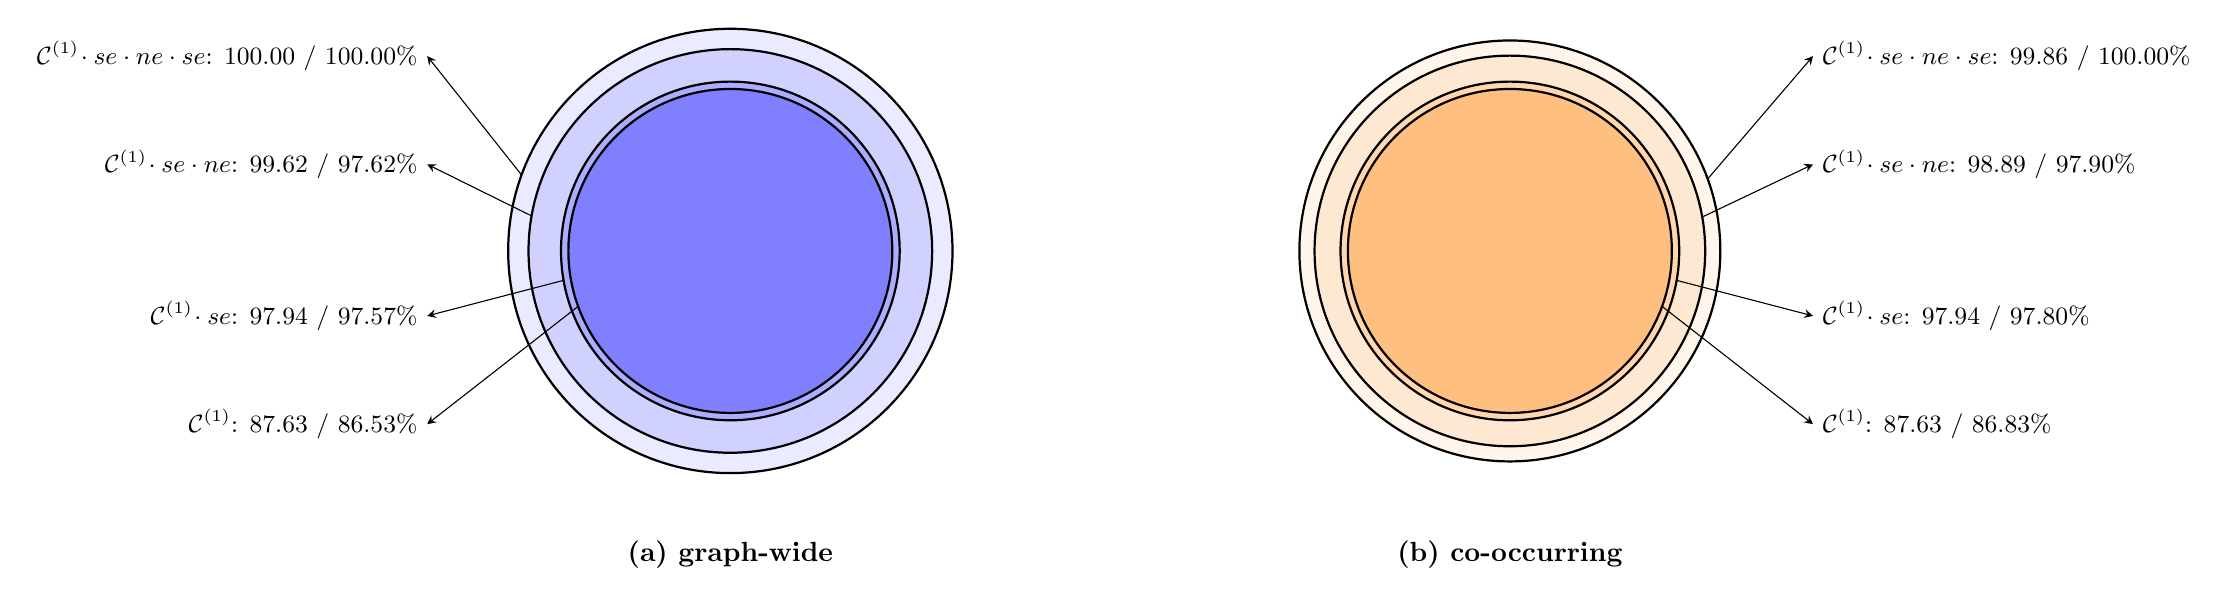
\begin{tikzpicture}[scale=0.55, every node/.style={font=\small}]
  % ============ LEFT PANEL: GRAPH-WIDE ============
  % Labels stacked vertically on the LEFT side of the panel
  \begin{scope}
    % Radii (gw): 3.74, 3.91, 4.66, 5.13
    \fill[blue!8]  (0,0) circle (5.13);
    \fill[blue!18] (0,0) circle (4.66);
    \fill[blue!32] (0,0) circle (3.91);
    \fill[blue!50] (0,0) circle (3.74);
    \draw[thick]   (0,0) circle (5.13);
    \draw[thick]   (0,0) circle (4.66);
    \draw[thick]   (0,0) circle (3.91);
    \draw[thick]   (0,0) circle (3.74);
    % Outer label at top-left, inner at bottom-left so leaders never cross.
    % Each circle's leader exits at its left edge at an angle.
    %   ne*se (5.13) -> label at (-9, 4.5)
    %   ne    (4.66) -> label at (-9, 2.0)
    %   se    (3.91) -> label at (-9,-1.5)
    %   CCD1  (3.74) -> label at (-9,-4.0)
    \draw[->,>=stealth] ({-5.13*cos(20)},{5.13*sin(20)}) -- (-7,4.5)
      node[anchor=east,align=right]
      {$\CC^{(1)}\!\cdot se\cdot ne\cdot se$: $100.00$ / $100.00\%$};
    \draw[->,>=stealth] ({-4.66*cos(10)},{4.66*sin(10)}) -- (-7,2.0)
      node[anchor=east,align=right]
      {$\CC^{(1)}\!\cdot se\cdot ne$: $99.62$ / $97.62\%$};
    \draw[->,>=stealth] ({-3.91*cos(10)},{-3.91*sin(10)}) -- (-7,-1.5)
      node[anchor=east,align=right]
      {$\CC^{(1)}\!\cdot se$: $97.94$ / $97.57\%$};
    \draw[->,>=stealth] ({-3.74*cos(20)},{-3.74*sin(20)}) -- (-7,-4.0)
      node[anchor=east,align=right]
      {$\CC^{(1)}$: $87.63$ / $86.53\%$};
    \node[font=\bfseries] at (0,-7) {(a) graph-wide};
  \end{scope}

  % ============ RIGHT PANEL: CO-OCCURRING ============
  % Labels stacked vertically on the RIGHT side of the panel
  \begin{scope}[xshift=18cm]
    % Radii (co): 3.74, 3.91, 4.51, 4.86
    \fill[orange!8]  (0,0) circle (4.86);
    \fill[orange!18] (0,0) circle (4.51);
    \fill[orange!32] (0,0) circle (3.91);
    \fill[orange!50] (0,0) circle (3.74);
    \draw[thick]     (0,0) circle (4.86);
    \draw[thick]     (0,0) circle (4.51);
    \draw[thick]     (0,0) circle (3.91);
    \draw[thick]     (0,0) circle (3.74);
    \draw[->,>=stealth] ({4.86*cos(20)},{4.86*sin(20)}) -- (7,4.5)
      node[anchor=west,align=left]
      {$\CC^{(1)}\!\cdot se\cdot ne\cdot se$: $99.86$ / $100.00\%$};
    \draw[->,>=stealth] ({4.51*cos(10)},{4.51*sin(10)}) -- (7,2.0)
      node[anchor=west,align=left]
      {$\CC^{(1)}\!\cdot se\cdot ne$: $98.89$ / $97.90\%$};
    \draw[->,>=stealth] ({3.91*cos(10)},{-3.91*sin(10)}) -- (7,-1.5)
      node[anchor=west,align=left]
      {$\CC^{(1)}\!\cdot se$: $97.94$ / $97.80\%$};
    \draw[->,>=stealth] ({3.74*cos(20)},{-3.74*sin(20)}) -- (7,-4.0)
      node[anchor=west,align=left]
      {$\CC^{(1)}$: $87.63$ / $86.83\%$};
    \node[font=\bfseries] at (0,-7) {(b) co-occurring};
  \end{scope}
\end{tikzpicture}%
}
\caption{Tree-space envelope at each pipeline stage on RSV2 (train: run~1,
$18{,}001$ trees; held out: run~2, same size). Areas are proportional to
$\log_{10} N_{\text{trees}}$ (so radii are proportional to $\sqrt{\log_{10} N}$).
Each circle is annotated with the fraction of held-out trees that fall inside
it (cumulative empirical coverage) and the model's cumulative probability mass
on trees inside that universe under the fitted $(\alpha,\beta)$. The two
quantities agree to within $\sim 2$ percentage points at every boundary in both
panels, despite each transition enlarging the tree count by many decimal orders
of magnitude.}
\label{fig:pipeline-venn}
\end{figure}

\paragraph{Held-out fit.}
We train the full pipeline on run~1 and grid-search $(\alpha,\beta)$ to maximise
the mean held-out log-probability on run~2 (no cross-validation needed: the two
runs are genuinely independent). The optima are
\begin{center}
\renewcommand{\arraystretch}{1.1}
\begin{tabular}{lrrrr}
\hline
mode & $\alpha^\star$ & $\beta^\star$ & mean $\log P$/tree & coverage \\
\hline
graph-wide   & $0.265$ & $0.0014$ & $-54.21$ & $18001/18001\ (100.0\%)$ \\
co-occurring & $0.260$ & $0.0084$ & $-54.11$ & $17976/18001\ \phantom{0}(99.86\%)$ \\
\hline
\end{tabular}
\end{center}
The graph-wide expansion covers every held-out tree; the $25$ co-occurring
misses are trees whose novel clades sit more than one NNI move away from any
clade-context in run~1, an SPR-scale rearrangement away.

\paragraph{Probability mass on NNI-expanded trees vs.\ empirical fraction.}
At the fitted $(\alpha,\beta)$, we compute in closed form the total probability
mass the model places on trees that contain at least one novel clade,
\begin{equation}
  P(\text{novel-clade tree}) \;=\; 1 - M(\rho),
  \qquad
  M(c) = \sum_{(L,R)\in S^{\text{obs}}(c)} \theta(L,R)\,M(L)\,M(R),
\end{equation}
restricted at every clade $c$ to the sub-sum over existing-only splits (novel
children contribute $M=0$). We then compare to the \emph{empirical} fraction of
held-out trees that actually contain a novel clade:
\begin{center}
\renewcommand{\arraystretch}{1.1}
\begin{tabular}{lrrr}
\hline
mode & model $P(\text{novel})$ & empirical & ratio \\
\hline
graph-wide   & $2.43\%$ & $2.06\%$ & $1.18\times$ \\
co-occurring & $2.20\%$ & $1.92\%$ & $1.15\times$ \\
\hline
\end{tabular}
\end{center}
The model overstates the speculative fraction by only $\sim 15$--$20\%$ in both
modes. Given that the universe of \emph{potentially} novel trees is $\sim
10^{40}$ times larger than the observed-clade tree set (cf.\ the table above),
matching the empirical novel-clade rate within a factor of $1.2$ is the
operative sense in which the NNI clade expansion is \emph{well-calibrated}: the
additive-$\alpha,\beta$ smoothing under the pipeline of
\eqref{eq:pipeline} carves a probability mass on the expansion zone that closely
tracks the rate at which independent posterior samples actually visit it.

\end{document}
